% !TEX program = lualatex
%!TEX TS-program = lualatex
\documentclass[12pt,a4paper]{article}
\usepackage{fontspec}
\usepackage{polyglossia}
\setdefaultlanguage{polish}
\usepackage{geometry}
\geometry{margin=2.1cm}
\usepackage[table]{xcolor}
\usepackage{longtable}
\usepackage{array}
\usepackage{booktabs}
\usepackage{enumitem}
\usepackage{ragged2e}
\usepackage{graphicx}
\usepackage{float}
\usepackage[hidelinks]{hyperref}
\usepackage{caption}
\definecolor{tableHeader}{HTML}{E8EEF7}
\definecolor{tableStripe}{HTML}{F7F9FC}
\definecolor{captionNote}{HTML}{4B5563}
\newcolumntype{L}[1]{>{\RaggedRight\arraybackslash}p{#1}}
\newcolumntype{C}[1]{>{\Centering\arraybackslash}p{#1}}
\newcommand{\opis}[1]{\par\smallskip{\small\color{captionNote}\itshape #1}\par}
\renewcommand{\arraystretch}{1.22}
\setlength{\tabcolsep}{4pt}
\setlist[itemize]{leftmargin=*, itemsep=2pt, topsep=2pt}
\setlength{\parindent}{0pt}
\setlength{\parskip}{6pt}
\graphicspath{{img/}{uml/}}
\emergencystretch=3em
\sloppy

\begin{document}

\begin{titlepage}
\centering
{\Large Dokumentacja projektu\par}
\vspace{1.2cm}
{\Huge\bfseries Calisia Banking App\par}
\vspace{0.5cm}
{\Large Aplikacja bankowa z panelem klienta, produktami finansowymi i modelem CQRS\par}
\vfill
{\large Data raportu: 06.06.2026\par}
\vspace{1cm}
{\large Autorzy:\par}
\vspace{0.2cm}
\begin{tabular}{c}
Kubryn Jeremiasz\\
Łaszuk Jakub\\
Makarevich Ksenia\\
Nuckowski Michał\\
Ruczyńska Nikola\\
Wołczko Jakub\\
Olszewski Dawid
\end{tabular}
\vfill
\end{titlepage}

\tableofcontents
\newpage

\section{Cel i zakres aplikacji}

Calisia Banking App jest aplikacją bankową przeznaczoną do obsługi podstawowych czynności klienta banku. System umożliwia rejestrację i logowanie klienta, prezentację dashboardu finansowego, zarządzanie produktami bankowymi, wykonywanie przelewów, obsługę kart oraz kredytu gotówkowego.

Aplikacja składa się z dwóch głównych części:
\begin{itemize}
\item frontendu typu SPA zbudowanego w React i TypeScript,
\item backendu REST API zbudowanego w .NET, podzielonego na warstwy API, Application, Domain, Infrastructure oraz ReadModel.
\end{itemize}

System korzysta z dwóch baz danych SQL Server. Baza zapisu \texttt{CalisiaWriteDb} przechowuje model domenowy oraz outbox, natomiast baza odczytu \texttt{CalisiaReadDb} przechowuje zoptymalizowane dane dashboardu.

\section{Najważniejsze funkcje systemu}

\rowcolors{2}{tableStripe}{white}
\begin{longtable}{L{4.1cm} L{11cm}}
\rowcolor{tableHeader}
\textbf{Obszar} & \textbf{Opis funkcjonalności}\\
\endhead
Rejestracja klienta & Utworzenie konta klienta, zahashowanie hasła oraz automatyczne dodanie produktów startowych: konta głównego i karty debetowej. Dla klienta prestiżowego tworzona jest także karta kredytowa.\\
Logowanie & Weryfikacja danych dostępowych i wydanie tokenu JWT używanego przez frontend do autoryzowanych żądań.\\
Dashboard & Prezentacja salda, listy produktów i historii zdarzeń finansowych. Dane pochodzą z modelu odczytu.\\
Produkty bankowe & Obsługa kont, kart oraz kredytów. Produkty są przechowywane w jednej tabeli \texttt{Products} z rozróżnieniem typu przez kolumnę \texttt{Discriminator}.\\
Przelewy & Obsługa przelewów własnych oraz zewnętrznych. Przelew własny aktualizuje saldo źródła i celu, a przelew zewnętrzny tylko obciąża konto źródłowe.\\
Kredyt gotówkowy & Dodanie produktu typu kredyt gotówkowy zwiększa saldo konta głównego. Wcześniejsza spłata pobiera kwotę kredytu z konta głównego i usuwa produkt kredytu.\\
Karty & Symulacja płatności kartą debetową pobiera środki z konta głównego. Symulacja płatności kartą kredytową zmniejsza dostępne saldo karty. Spłata karty kredytowej pobiera z konta głównego wykorzystany limit.\\
\end{longtable}

\section{Architektura}

Backend stosuje podział zbliżony do Clean Architecture. Warstwa API odpowiada za kontrolery HTTP i autoryzację, Application za przypadki użycia, Domain za reguły biznesowe, Infrastructure za dostęp do bazy, JWT i outbox, a ReadModel za projekcje dashboardu.

\begin{figure}[H]
\centering
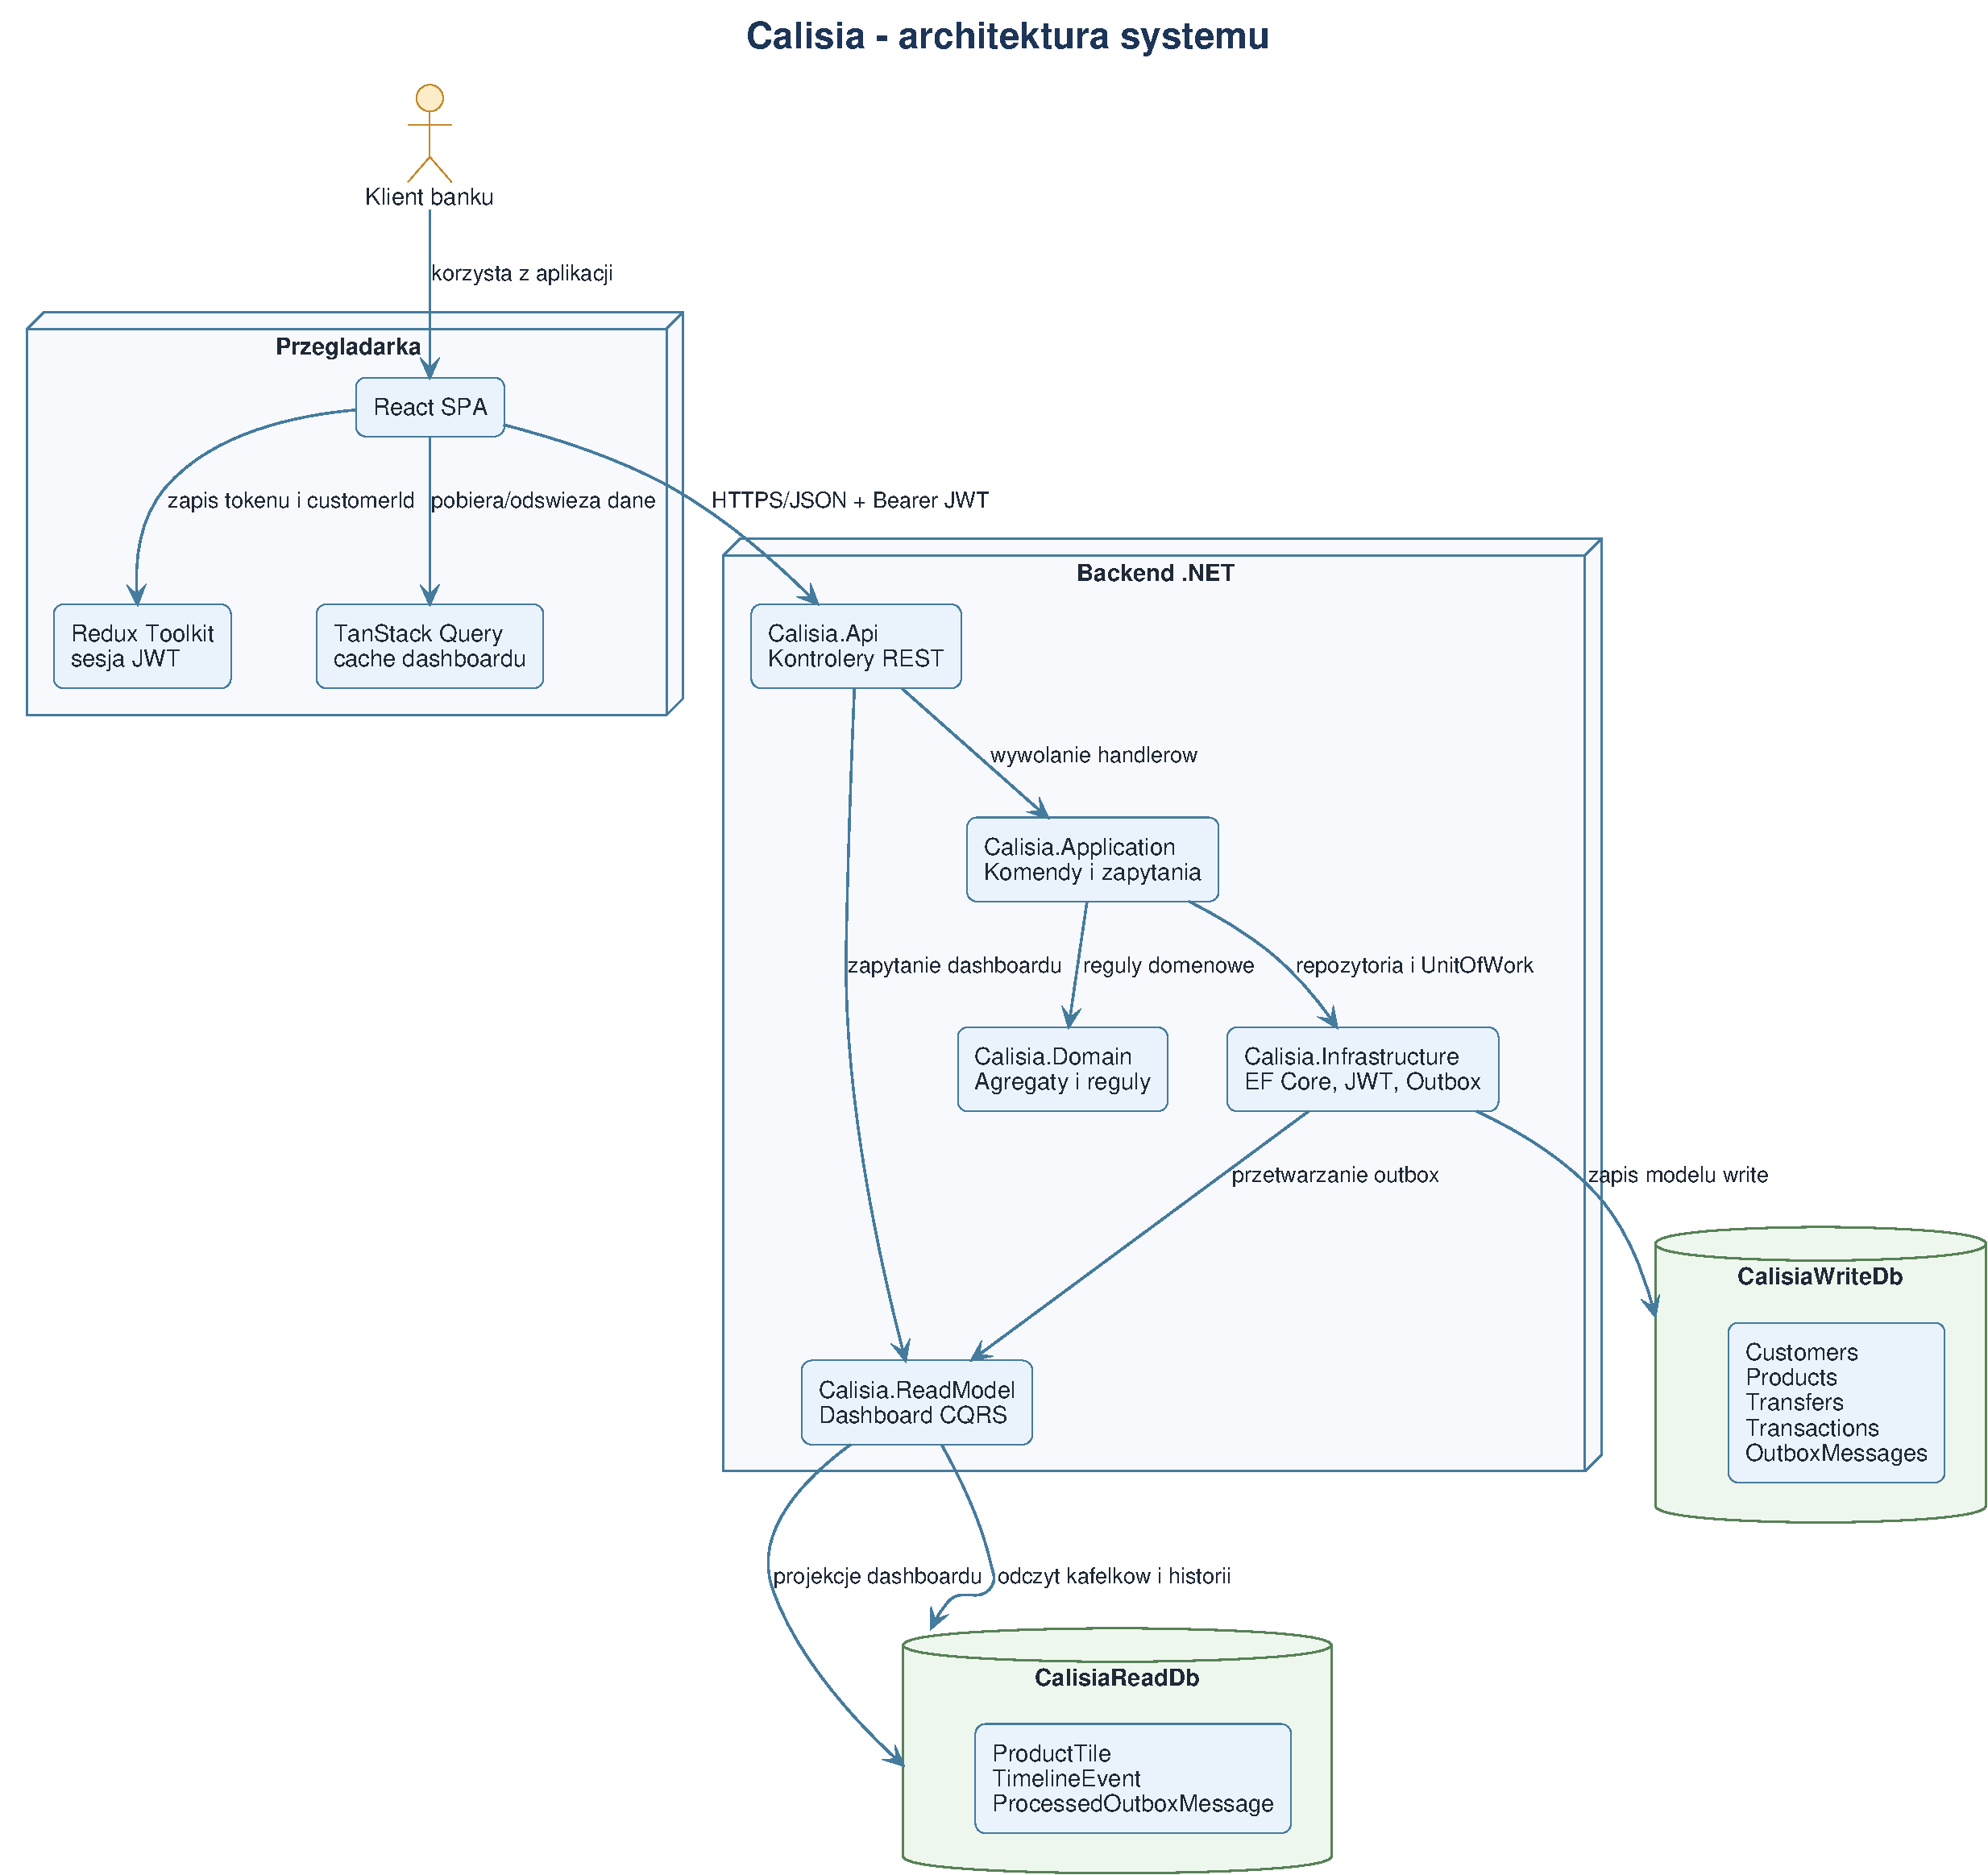
\includegraphics[width=\textwidth,height=0.78\textheight,keepaspectratio]{uml/01_architektura_systemu.pdf}
\caption{Architektura systemu Calisia}
\opis{Diagram przedstawia główne moduły systemu, przepływ żądań z aplikacji React do API oraz rozdzielenie bazy zapisu i bazy odczytu.}
\end{figure}

\subsection{Warstwy backendu}

\rowcolors{2}{tableStripe}{white}
\begin{longtable}{L{4cm} L{11.1cm}}
\rowcolor{tableHeader}
\textbf{Warstwa} & \textbf{Odpowiedzialność}\\
\endhead
\texttt{Calisia.Api} & Kontrolery REST, middleware obsługi wyjątków, konfiguracja CORS, JWT i Swagger/OpenAPI.\\
\texttt{Calisia.Contracts} & Kontrakty żądań i odpowiedzi HTTP, między innymi rejestracja, logowanie, produkty, karty i przelewy.\\
\texttt{Calisia.Application} & Komendy i zapytania aplikacyjne, walidacja przypadków użycia oraz koordynacja repozytoriów i jednostki pracy.\\
\texttt{Calisia.Domain} & Agregaty, encje, value objects, enumy i zdarzenia domenowe.\\
\texttt{Calisia.Infrastructure} & Implementacje repozytoriów EF Core, konfiguracje mapowania, hashowanie haseł, tokeny JWT oraz procesor outbox.\\
\texttt{Calisia.ReadModel} & Odczyt dashboardu, modele \texttt{ProductTile} i \texttt{TimelineEvent} oraz projekcje zdarzeń domenowych.\\
\end{longtable}

\section{Przypadki użycia}

Diagram przypadków użycia pokazuje czynności dostępne dla gościa oraz zalogowanego klienta.

\begin{figure}[H]
\centering
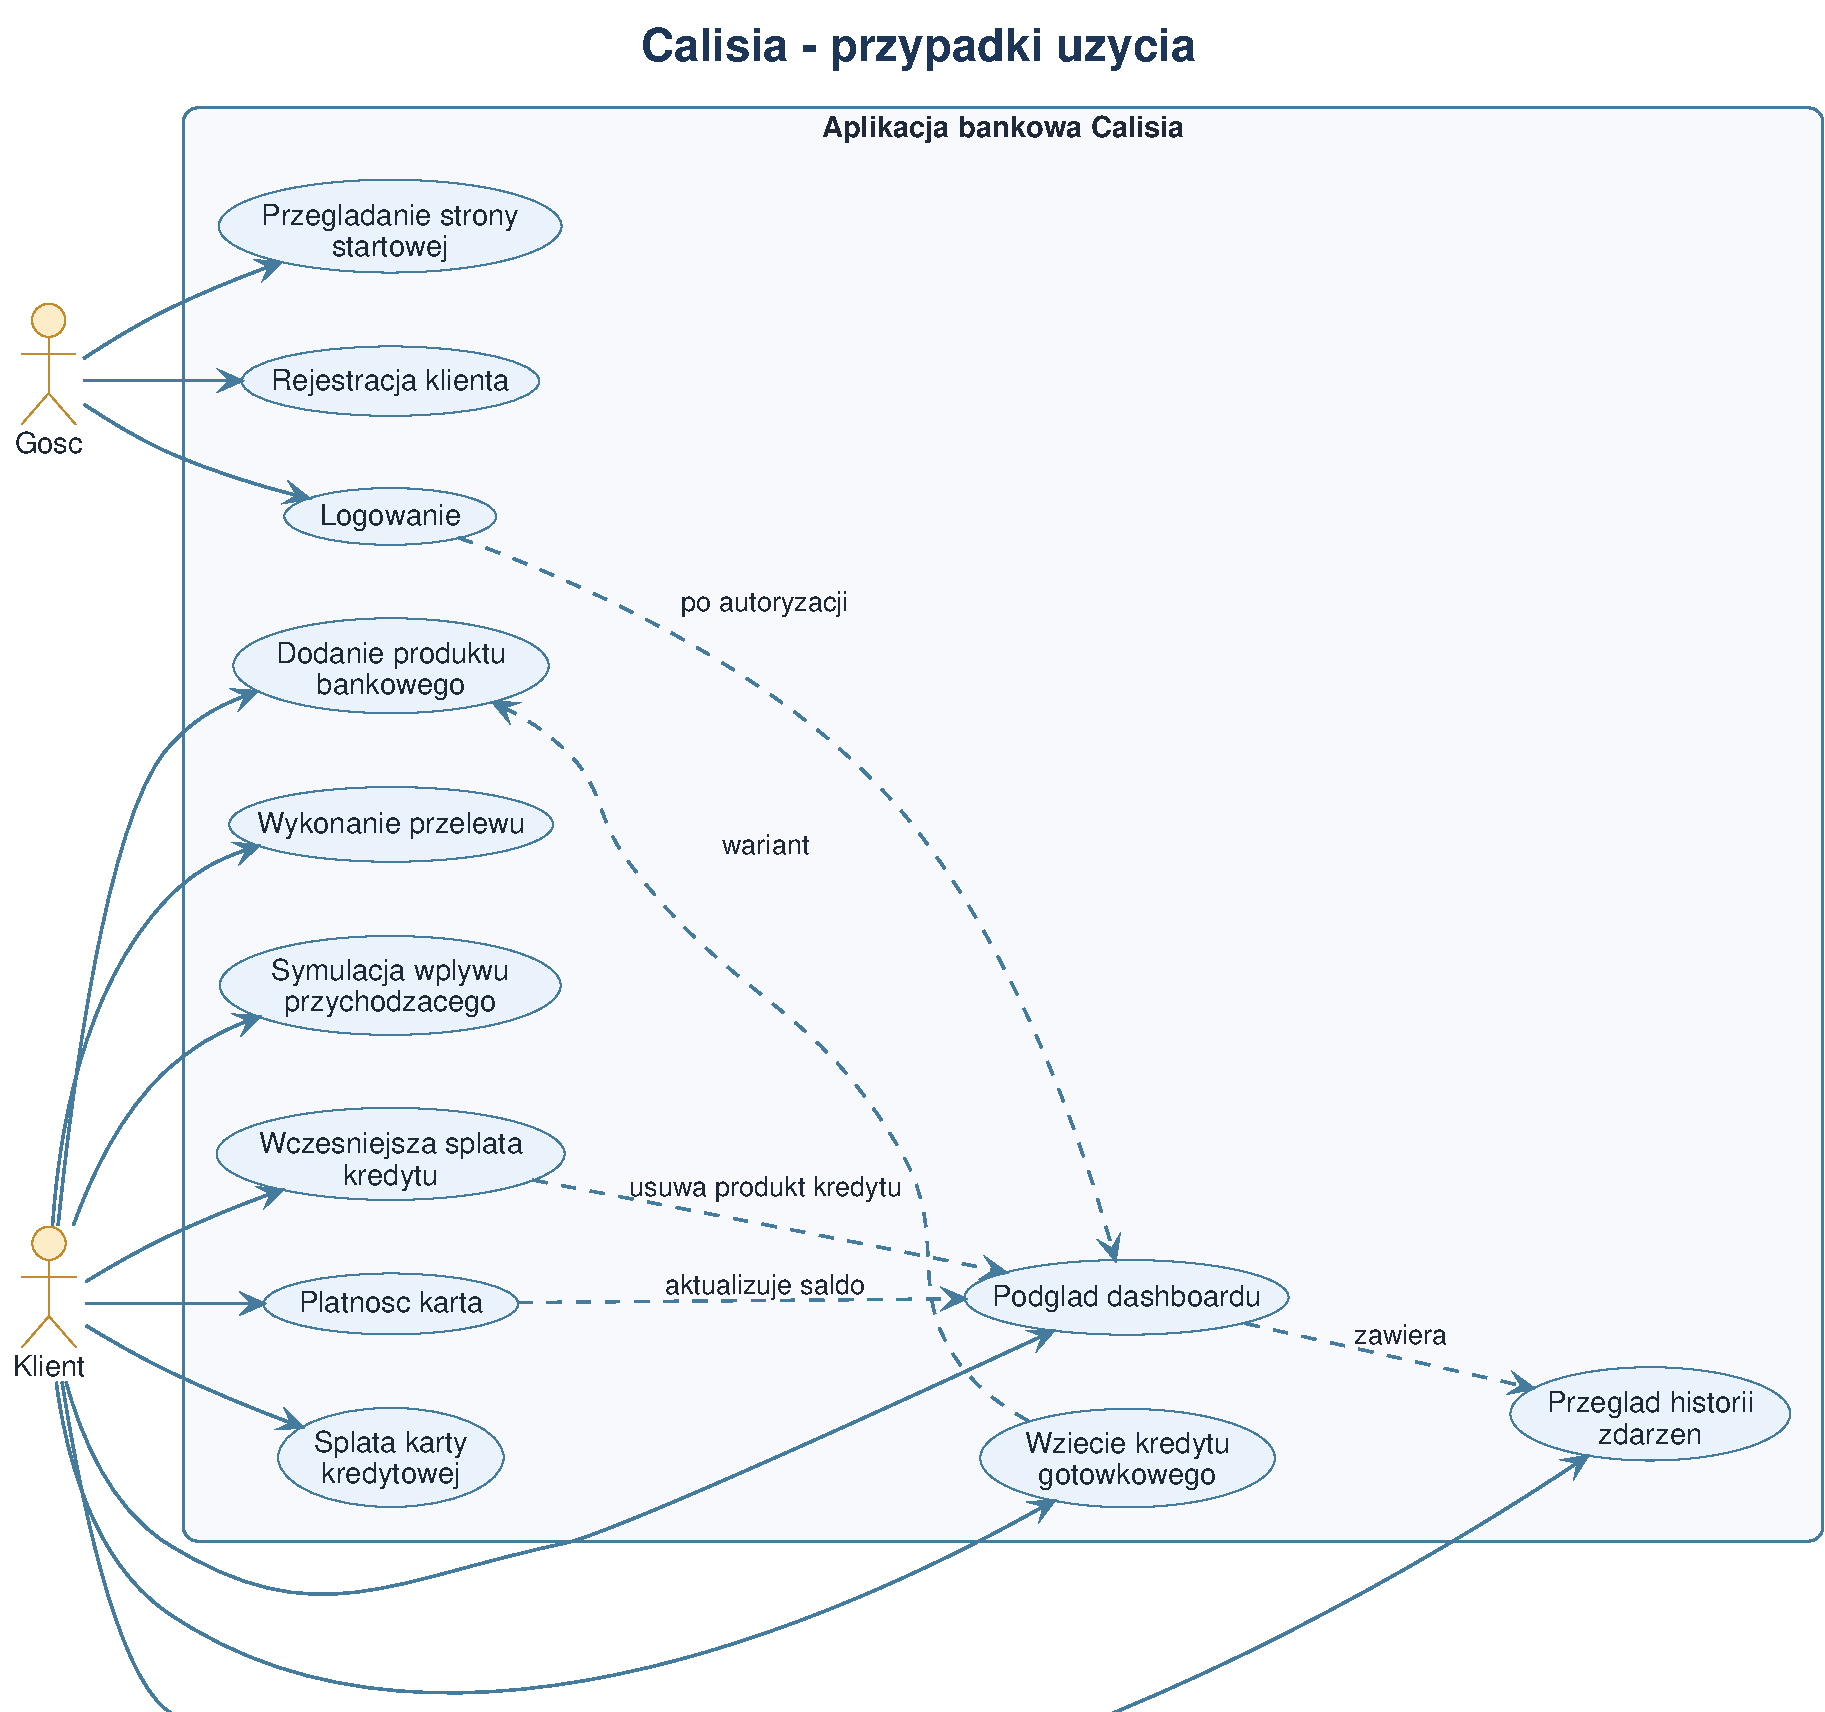
\includegraphics[width=\textwidth,height=0.78\textheight,keepaspectratio]{uml/02_przypadki_uzycia.pdf}
\caption{Przypadki użycia aplikacji}
\opis{Diagram pokazuje funkcje dostępne dla gościa oraz operacje wykonywane po zalogowaniu klienta banku.}
\end{figure}

\section{Model domenowy}

Centralnym elementem domeny jest abstrakcyjny produkt bankowy \texttt{Product}. Dziedziczą po nim: \texttt{BankAccount}, \texttt{Card} i \texttt{Loan}. Takie podejście pozwala przechowywać różne produkty finansowe w jednej tabeli, przy zachowaniu osobnych reguł biznesowych dla kont, kart i kredytów.

\begin{figure}[H]
\centering
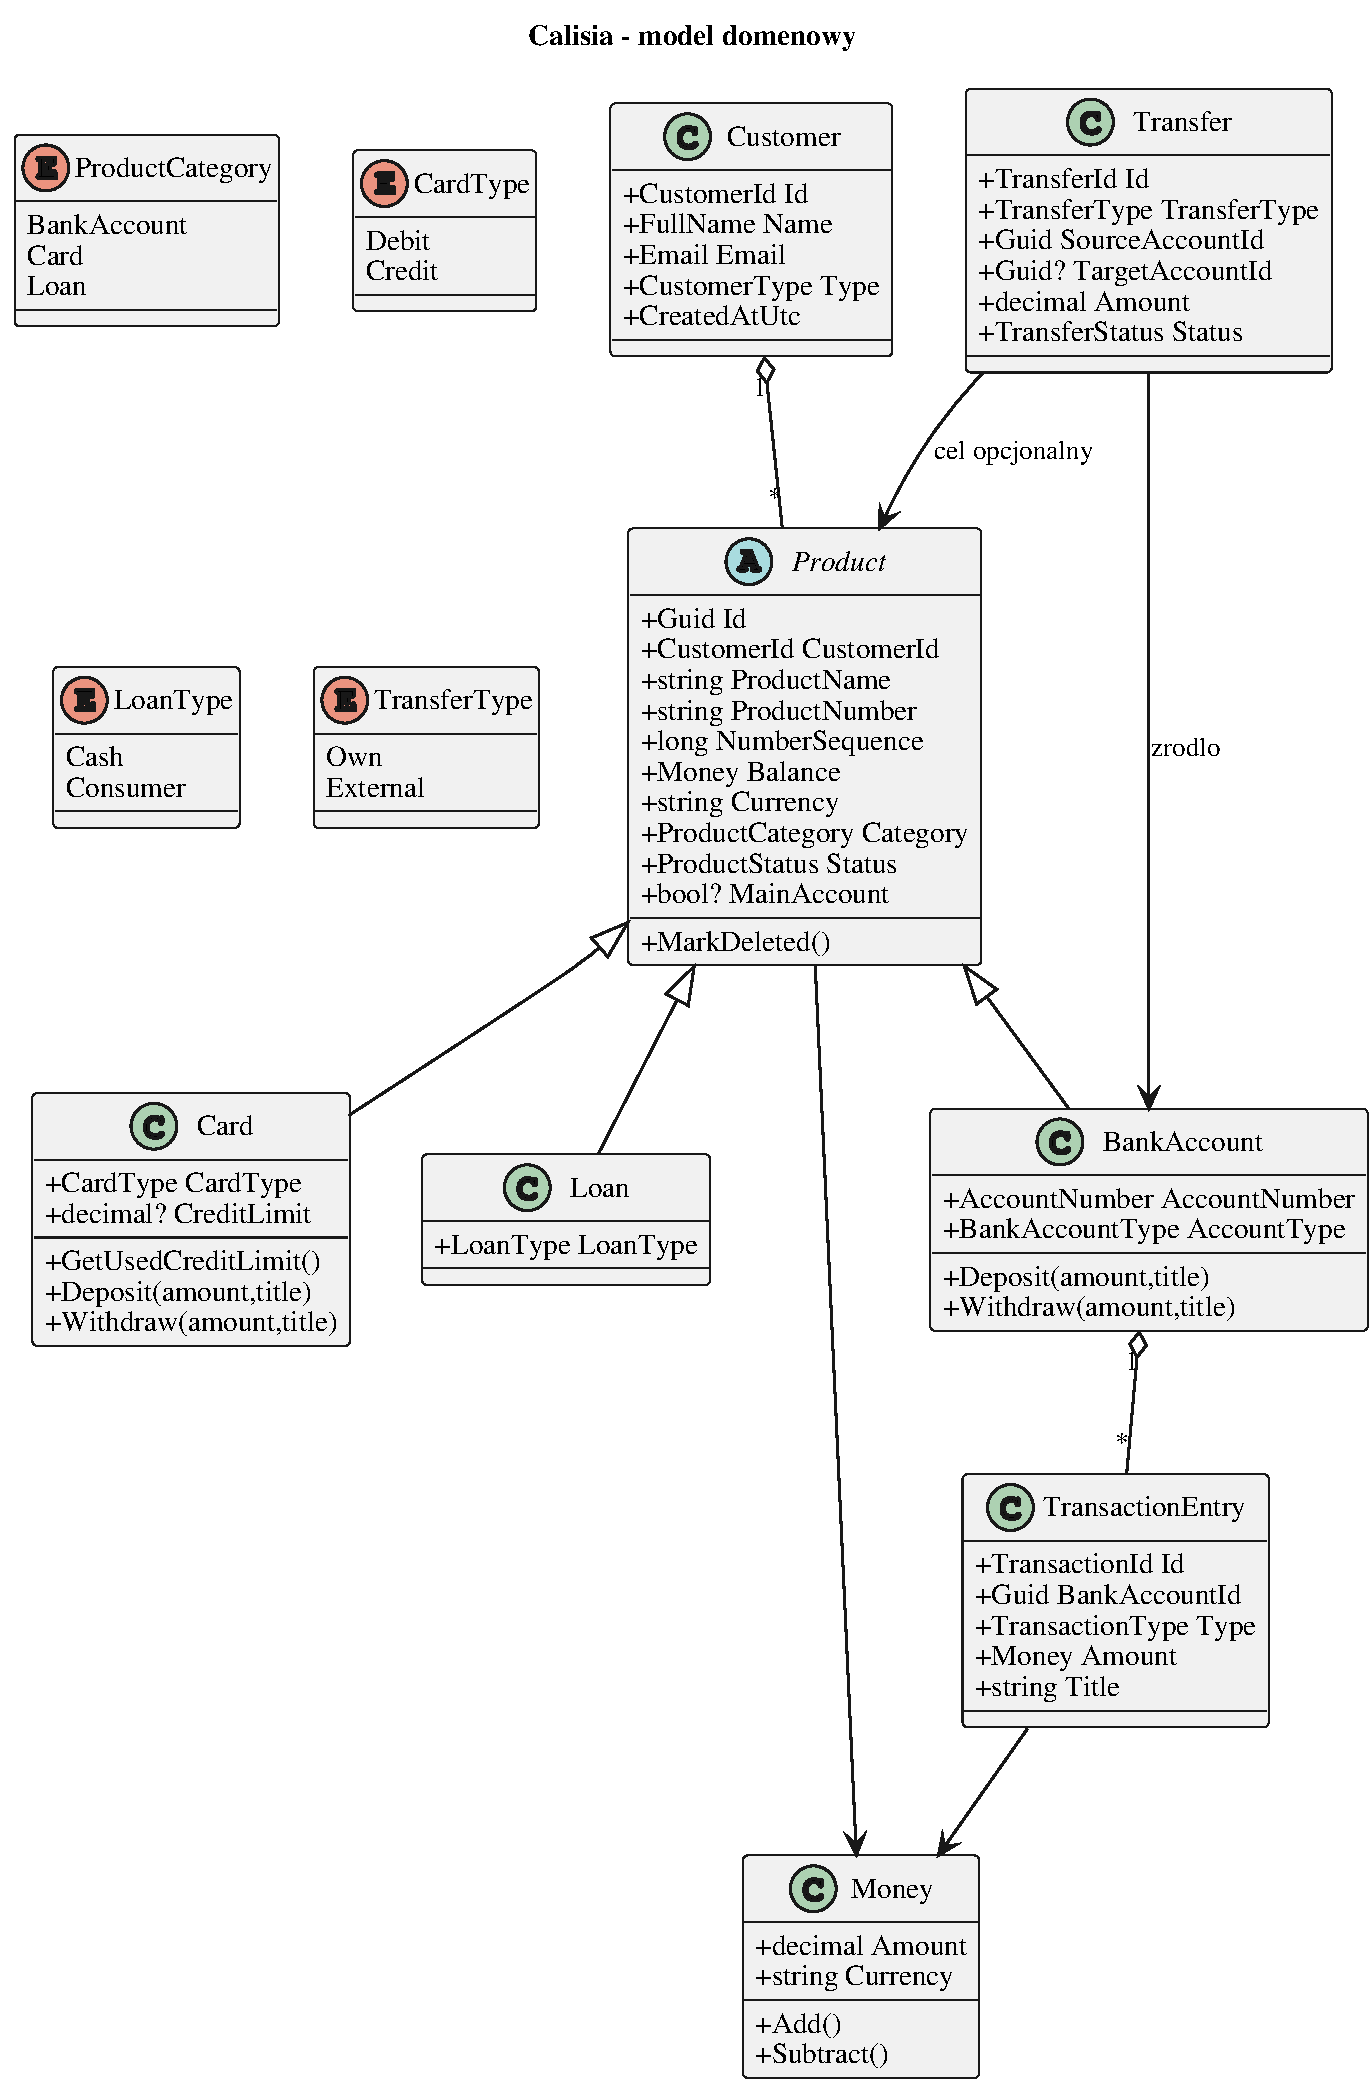
\includegraphics[width=\textwidth,height=0.72\textheight,keepaspectratio]{uml/03_model_domenowy.pdf}
\caption{Model domenowy}
\opis{Diagram prezentuje najważniejsze agregaty domenowe: klienta, produkty bankowe, przelewy, transakcje oraz obiekt wartości pieniędzy.}
\end{figure}

\subsection{Wybrane reguły domenowe}

\begin{itemize}
\item Konto bankowe może przyjmować wpłaty i wypłaty, a każda operacja generuje wpis transakcji oraz zdarzenie domenowe.
\item Karta debetowa nie posiada limitu kredytowego i przy płatności obciąża konto główne klienta.
\item Karta kredytowa posiada \texttt{CreditLimit}; jej saldo reprezentuje dostępny limit. Płatność zmniejsza saldo karty, a spłata zwiększa je do wysokości limitu.
\item Kredyt gotówkowy jest produktem typu \texttt{Loan}. Wzięcie kredytu zasila konto główne, natomiast wcześniejsza spłata pobiera kwotę kredytu z konta głównego i usuwa produkt kredytu.
\item Przelew własny aktualizuje dwa produkty: źródłowy i docelowy. Przelew zewnętrzny aktualizuje tylko produkt źródłowy.
\end{itemize}

\section{Schemat bazy danych}

System korzysta z dwóch baz: zapisu i odczytu. Baza zapisu przechowuje pełny stan domenowy, a baza odczytu przechowuje uproszczony widok potrzebny dashboardowi.

\begin{figure}[H]
\centering
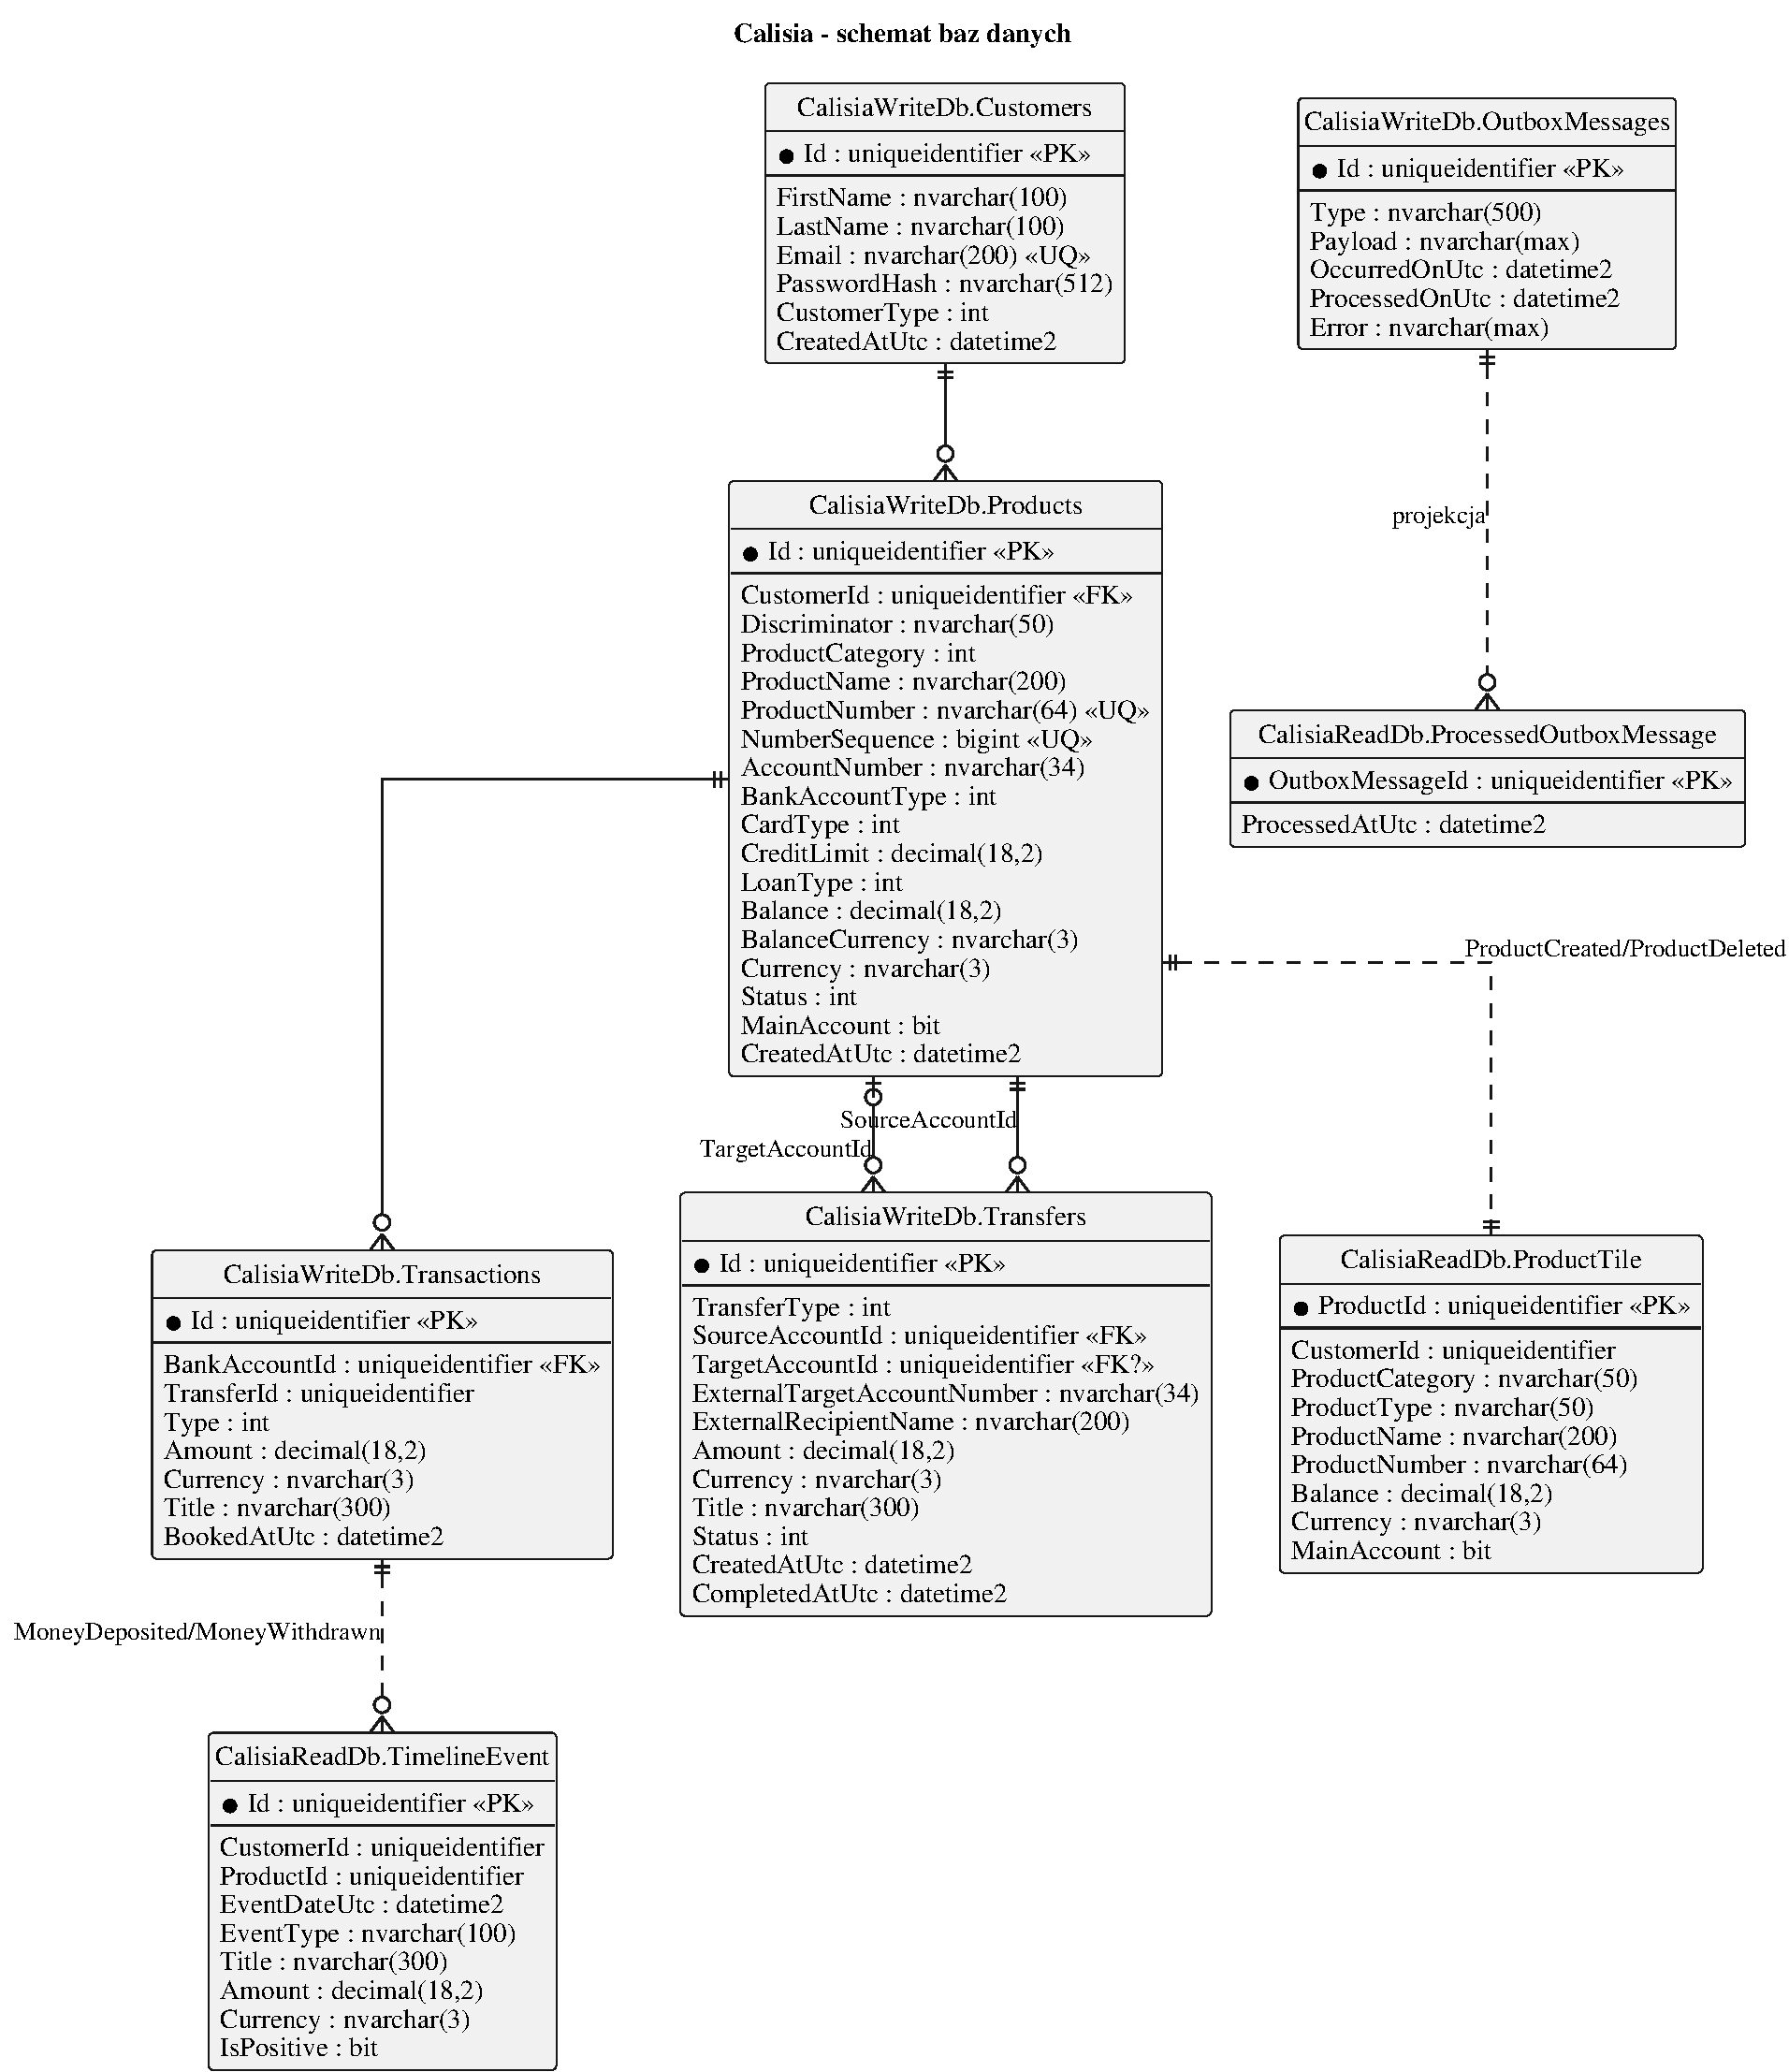
\includegraphics[width=\textwidth,height=0.72\textheight,keepaspectratio]{uml/04_erd_baza_danych.pdf}
\caption{Schemat baz danych write/read}
\opis{Diagram opisuje relacje między tabelami modelu zapisu oraz tabelami projekcji dashboardu w modelu odczytu.}
\end{figure}

\subsection{CalisiaWriteDb}

\rowcolors{2}{tableStripe}{white}
\begin{longtable}{L{4cm} L{11.1cm}}
\rowcolor{tableHeader}
\textbf{Tabela} & \textbf{Znaczenie}\\
\endhead
\texttt{Customers} & Dane klienta, email, hash hasła, typ klienta oraz data utworzenia.\\
\texttt{Products} & Wspólna tabela produktów bankowych. Kolumna \texttt{Discriminator} rozróżnia konto, kartę i kredyt.\\
\texttt{Transactions} & Historia operacji na kontach bankowych.\\
\texttt{Transfers} & Dane przelewów własnych i zewnętrznych.\\
\texttt{OutboxMessages} & Zdarzenia domenowe oczekujące na projekcję do bazy odczytu.\\
\end{longtable}

\subsection{CalisiaReadDb}

\rowcolors{2}{tableStripe}{white}
\begin{longtable}{L{4cm} L{11.1cm}}
\rowcolor{tableHeader}
\textbf{Tabela} & \textbf{Znaczenie}\\
\endhead
\texttt{ProductTile} & Kafelki produktów widoczne na dashboardzie: typ, numer, saldo, waluta i oznaczenie konta głównego.\\
\texttt{TimelineEvent} & Historia zdarzeń finansowych prezentowana w panelu użytkownika.\\
\texttt{ProcessedOutboxMessage} & Rejestr przetworzonych wiadomości outbox, chroniący przed podwójną projekcją.\\
\end{longtable}

\section{API REST}

\begin{figure}[H]
\centering
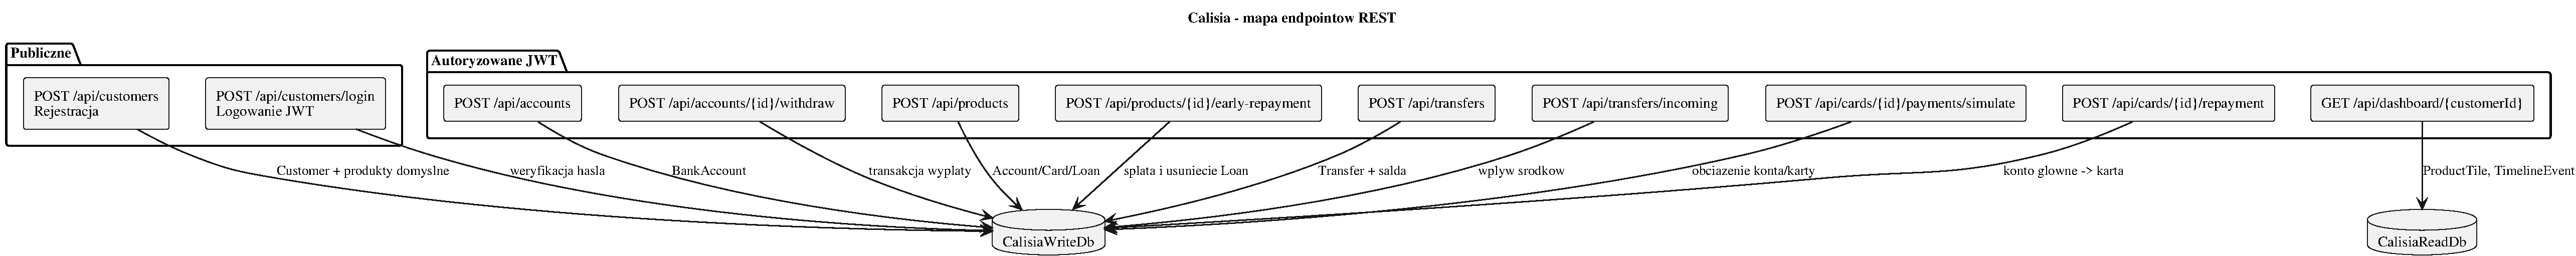
\includegraphics[width=\textwidth,height=0.78\textheight,keepaspectratio]{uml/06_endpointy_api.pdf}
\caption{Mapa endpointów API}
\opis{Diagram porządkuje endpointy REST według obszarów funkcjonalnych i wskazuje, które bazy danych są przez nie wykorzystywane.}
\end{figure}

\rowcolors{2}{tableStripe}{white}
\begin{longtable}{L{5.2cm} L{10cm}}
\rowcolor{tableHeader}
\textbf{Endpoint} & \textbf{Opis}\\
\endhead
\texttt{POST /api/customers} & Rejestracja klienta.\\
\texttt{POST /api/customers/login} & Logowanie i wydanie JWT.\\
\texttt{GET /api/dashboard/\{customerId\}} & Pobranie danych dashboardu z modelu odczytu.\\
\texttt{POST /api/accounts} & Otwarcie nowego konta bankowego.\\
\texttt{POST /api/accounts/\{id\}/withdraw} & Wypłata środków z konta.\\
\texttt{POST /api/products} & Dodanie produktu bankowego: konto, karta lub kredyt.\\
\texttt{POST /api/products/\{id\}/early-repayment} & Wcześniejsza spłata kredytu gotówkowego.\\
\texttt{POST /api/transfers} & Utworzenie przelewu własnego lub zewnętrznego.\\
\texttt{POST /api/transfers/incoming} & Symulacja wpływu przychodzącego.\\
\texttt{POST /api/cards/\{id\}/payments/simulate} & Symulacja płatności kartą debetową lub kredytową.\\
\texttt{POST /api/cards/\{id\}/repayment} & Spłata wykorzystanego limitu karty kredytowej.\\
\end{longtable}

\section{Frontend}

Frontend jest aplikacją React SPA. Routing realizuje \texttt{AppRouter}, stan sesji przechowywany jest w Redux Toolkit, a pobieranie i odświeżanie danych dashboardu obsługuje TanStack Query.

\begin{figure}[H]
\centering
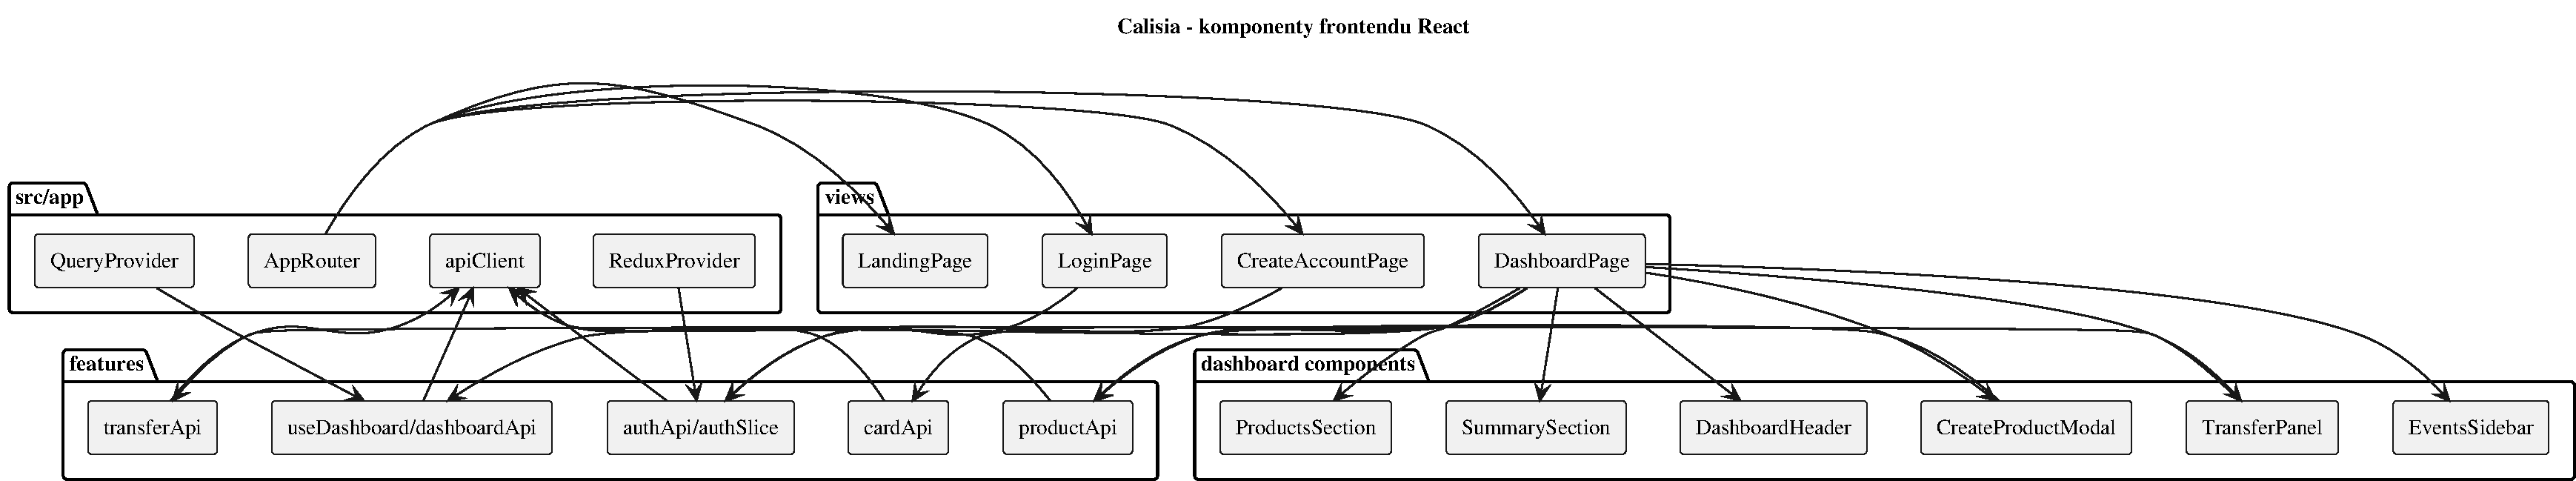
\includegraphics[width=\textwidth,height=0.78\textheight,keepaspectratio]{uml/05_frontend_komponenty.pdf}
\caption{Komponenty frontendu}
\opis{Diagram pokazuje zależności między routingiem, widokami, komponentami dashboardu oraz warstwą komunikacji z API.}
\end{figure}

\subsection{Ekrany aplikacji}

\begin{figure}[H]
\centering

\includegraphics[width=\textwidth]{\detokenize{img/Landing Page.png}}
\caption{Strona startowa aplikacji}
\opis{Ekran wejściowy prezentuje markę Calisia i prowadzi użytkownika do logowania albo rejestracji nowego klienta.}
\end{figure}

\begin{figure}[H]
\centering

\includegraphics[width=0.86\textwidth]{\detokenize{img/Rejestracja klienta.png}}
\caption{Formularz rejestracji klienta}
\opis{Formularz zbiera podstawowe dane klienta oraz typ klienta, na podstawie którego backend tworzy produkty startowe.}
\end{figure}

\begin{figure}[H]
\centering
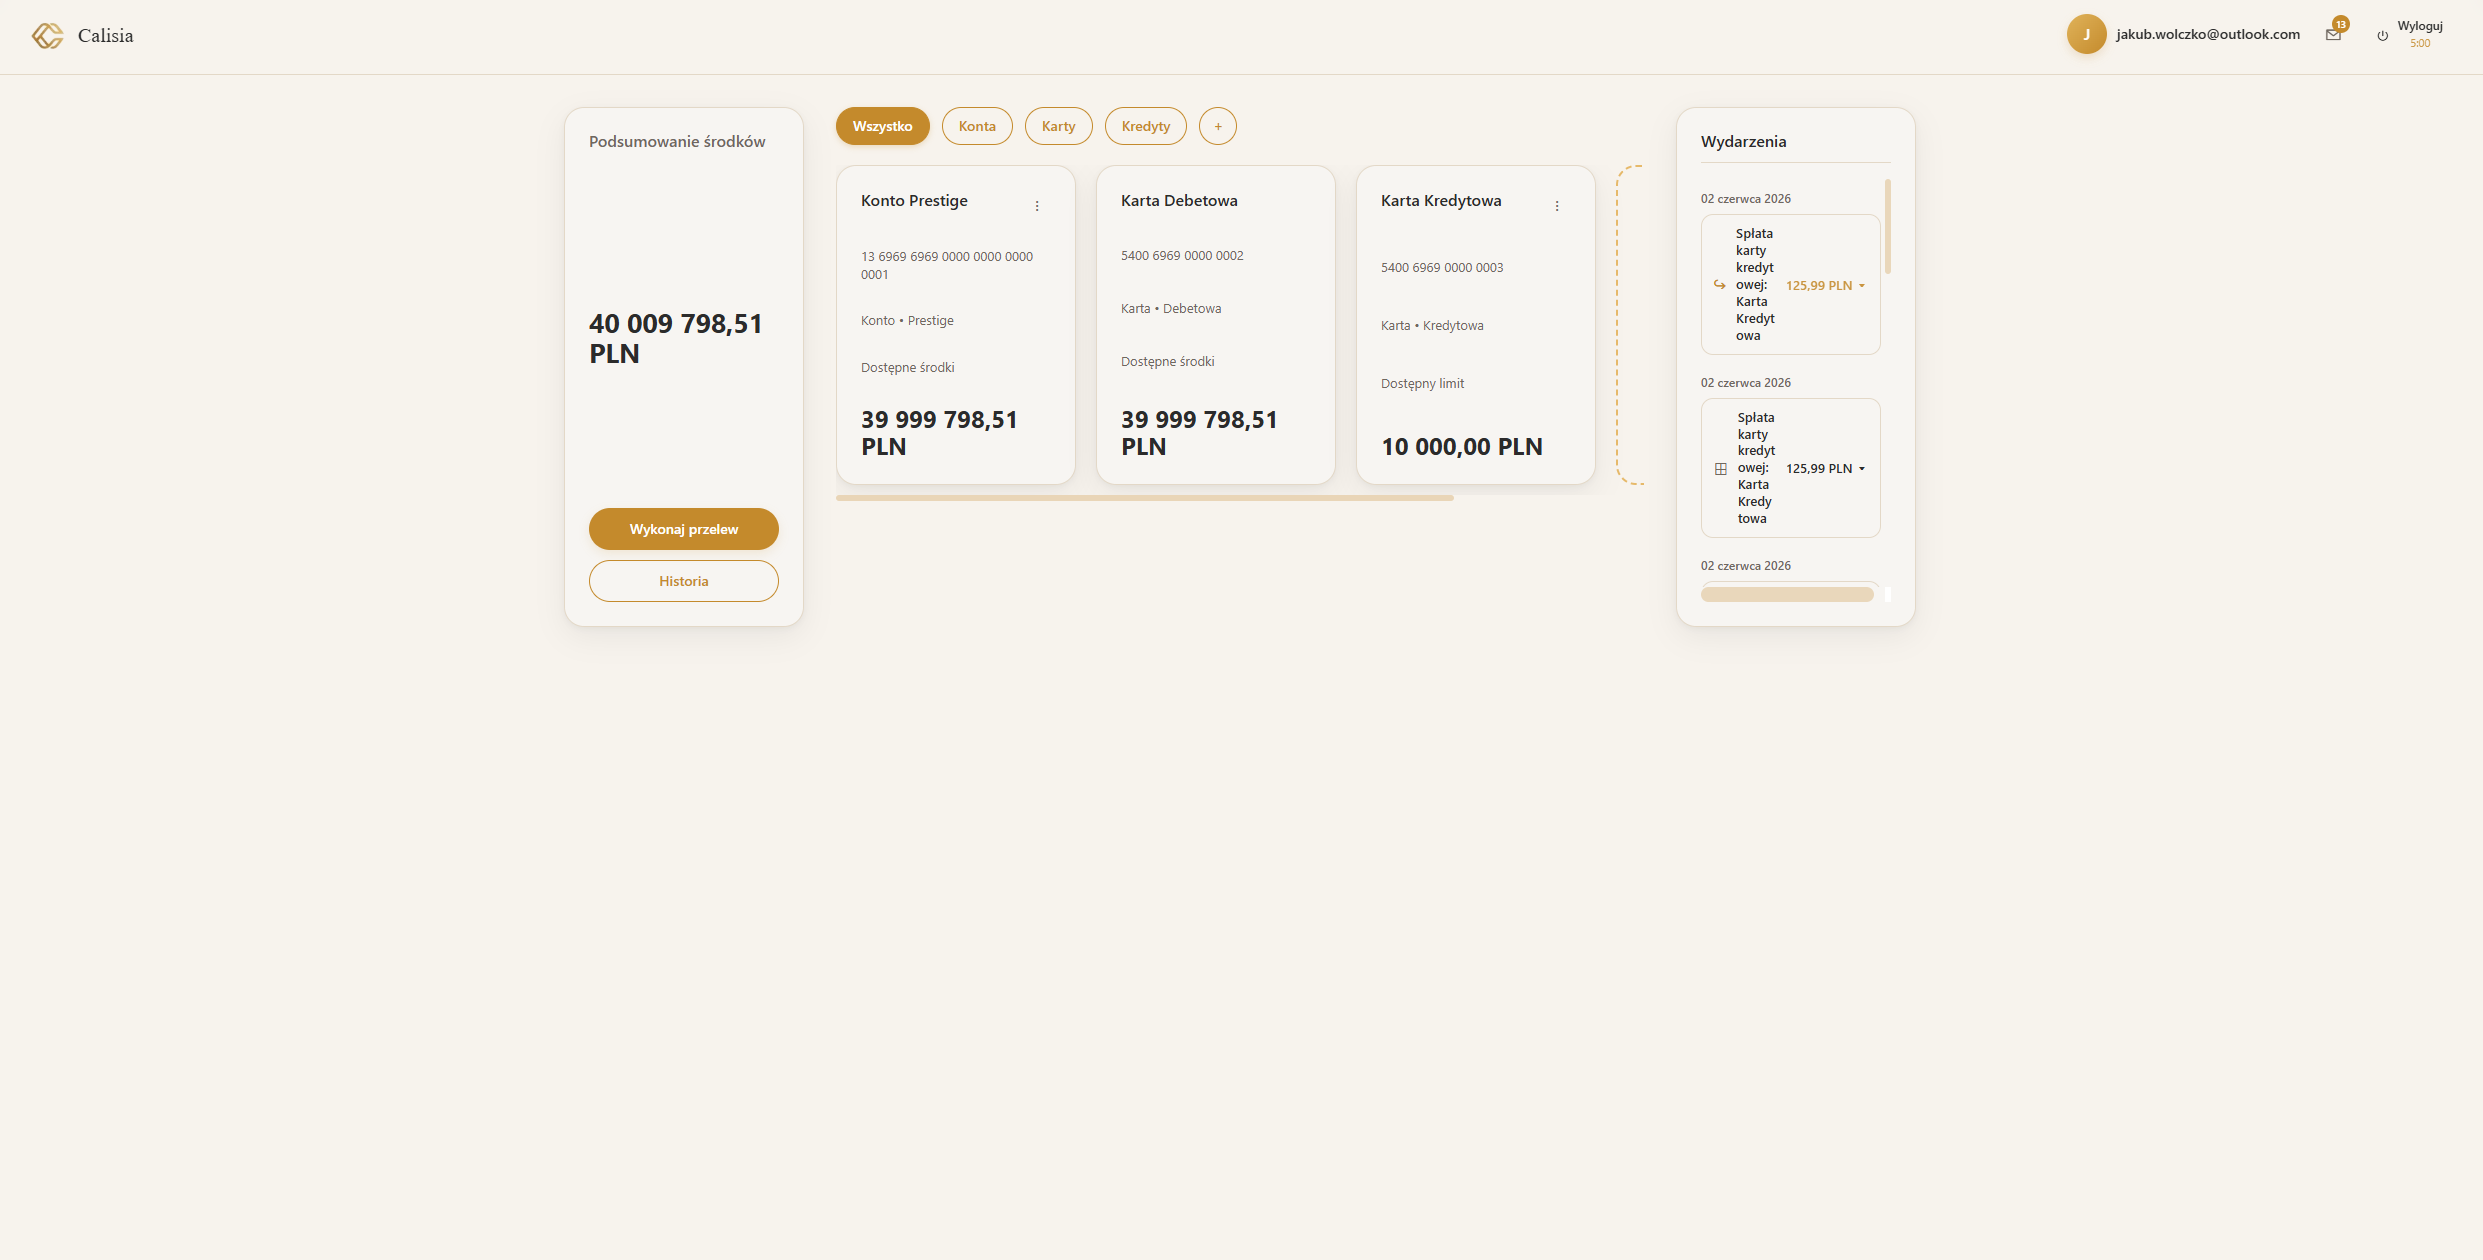
\includegraphics[width=\textwidth]{img/Dashboard.png}
\caption{Dashboard klienta}
\opis{Dashboard jest głównym widokiem roboczym klienta: prezentuje saldo, produkty, szybkie akcje i historię zdarzeń.}
\end{figure}

\begin{figure}[H]
\centering

\includegraphics[width=0.86\textwidth]{\detokenize{img/Nowy przelew.png}}
\caption{Panel tworzenia przelewu}
\opis{Panel umożliwia wykonanie przelewu własnego lub zewnętrznego z walidacją konta źródłowego, odbiorcy, tytułu i kwoty.}
\end{figure}

\begin{figure}[H]
\centering

\includegraphics[width=0.86\textwidth]{\detokenize{img/Nowy Produkt - Kredyt.png}}
\caption{Dodanie produktu typu kredyt gotówkowy}
\opis{Modal produktu pozwala wybrać kredyt gotówkowy i podać wnioskowaną kwotę, która po zatwierdzeniu zasila konto główne.}
\end{figure}

\begin{figure}[H]
\centering

\includegraphics[width=\textwidth]{\detokenize{img/Historia transakcji.png}}
\caption{Historia transakcji i zdarzeń}
\opis{Widok historii pokazuje zdarzenia finansowe generowane przez przelewy, wpłaty, wypłaty, płatności kartą i spłaty.}
\end{figure}

\section{Przepływy procesów}

\subsection{Rejestracja i logowanie}

\begin{figure}[H]
\centering
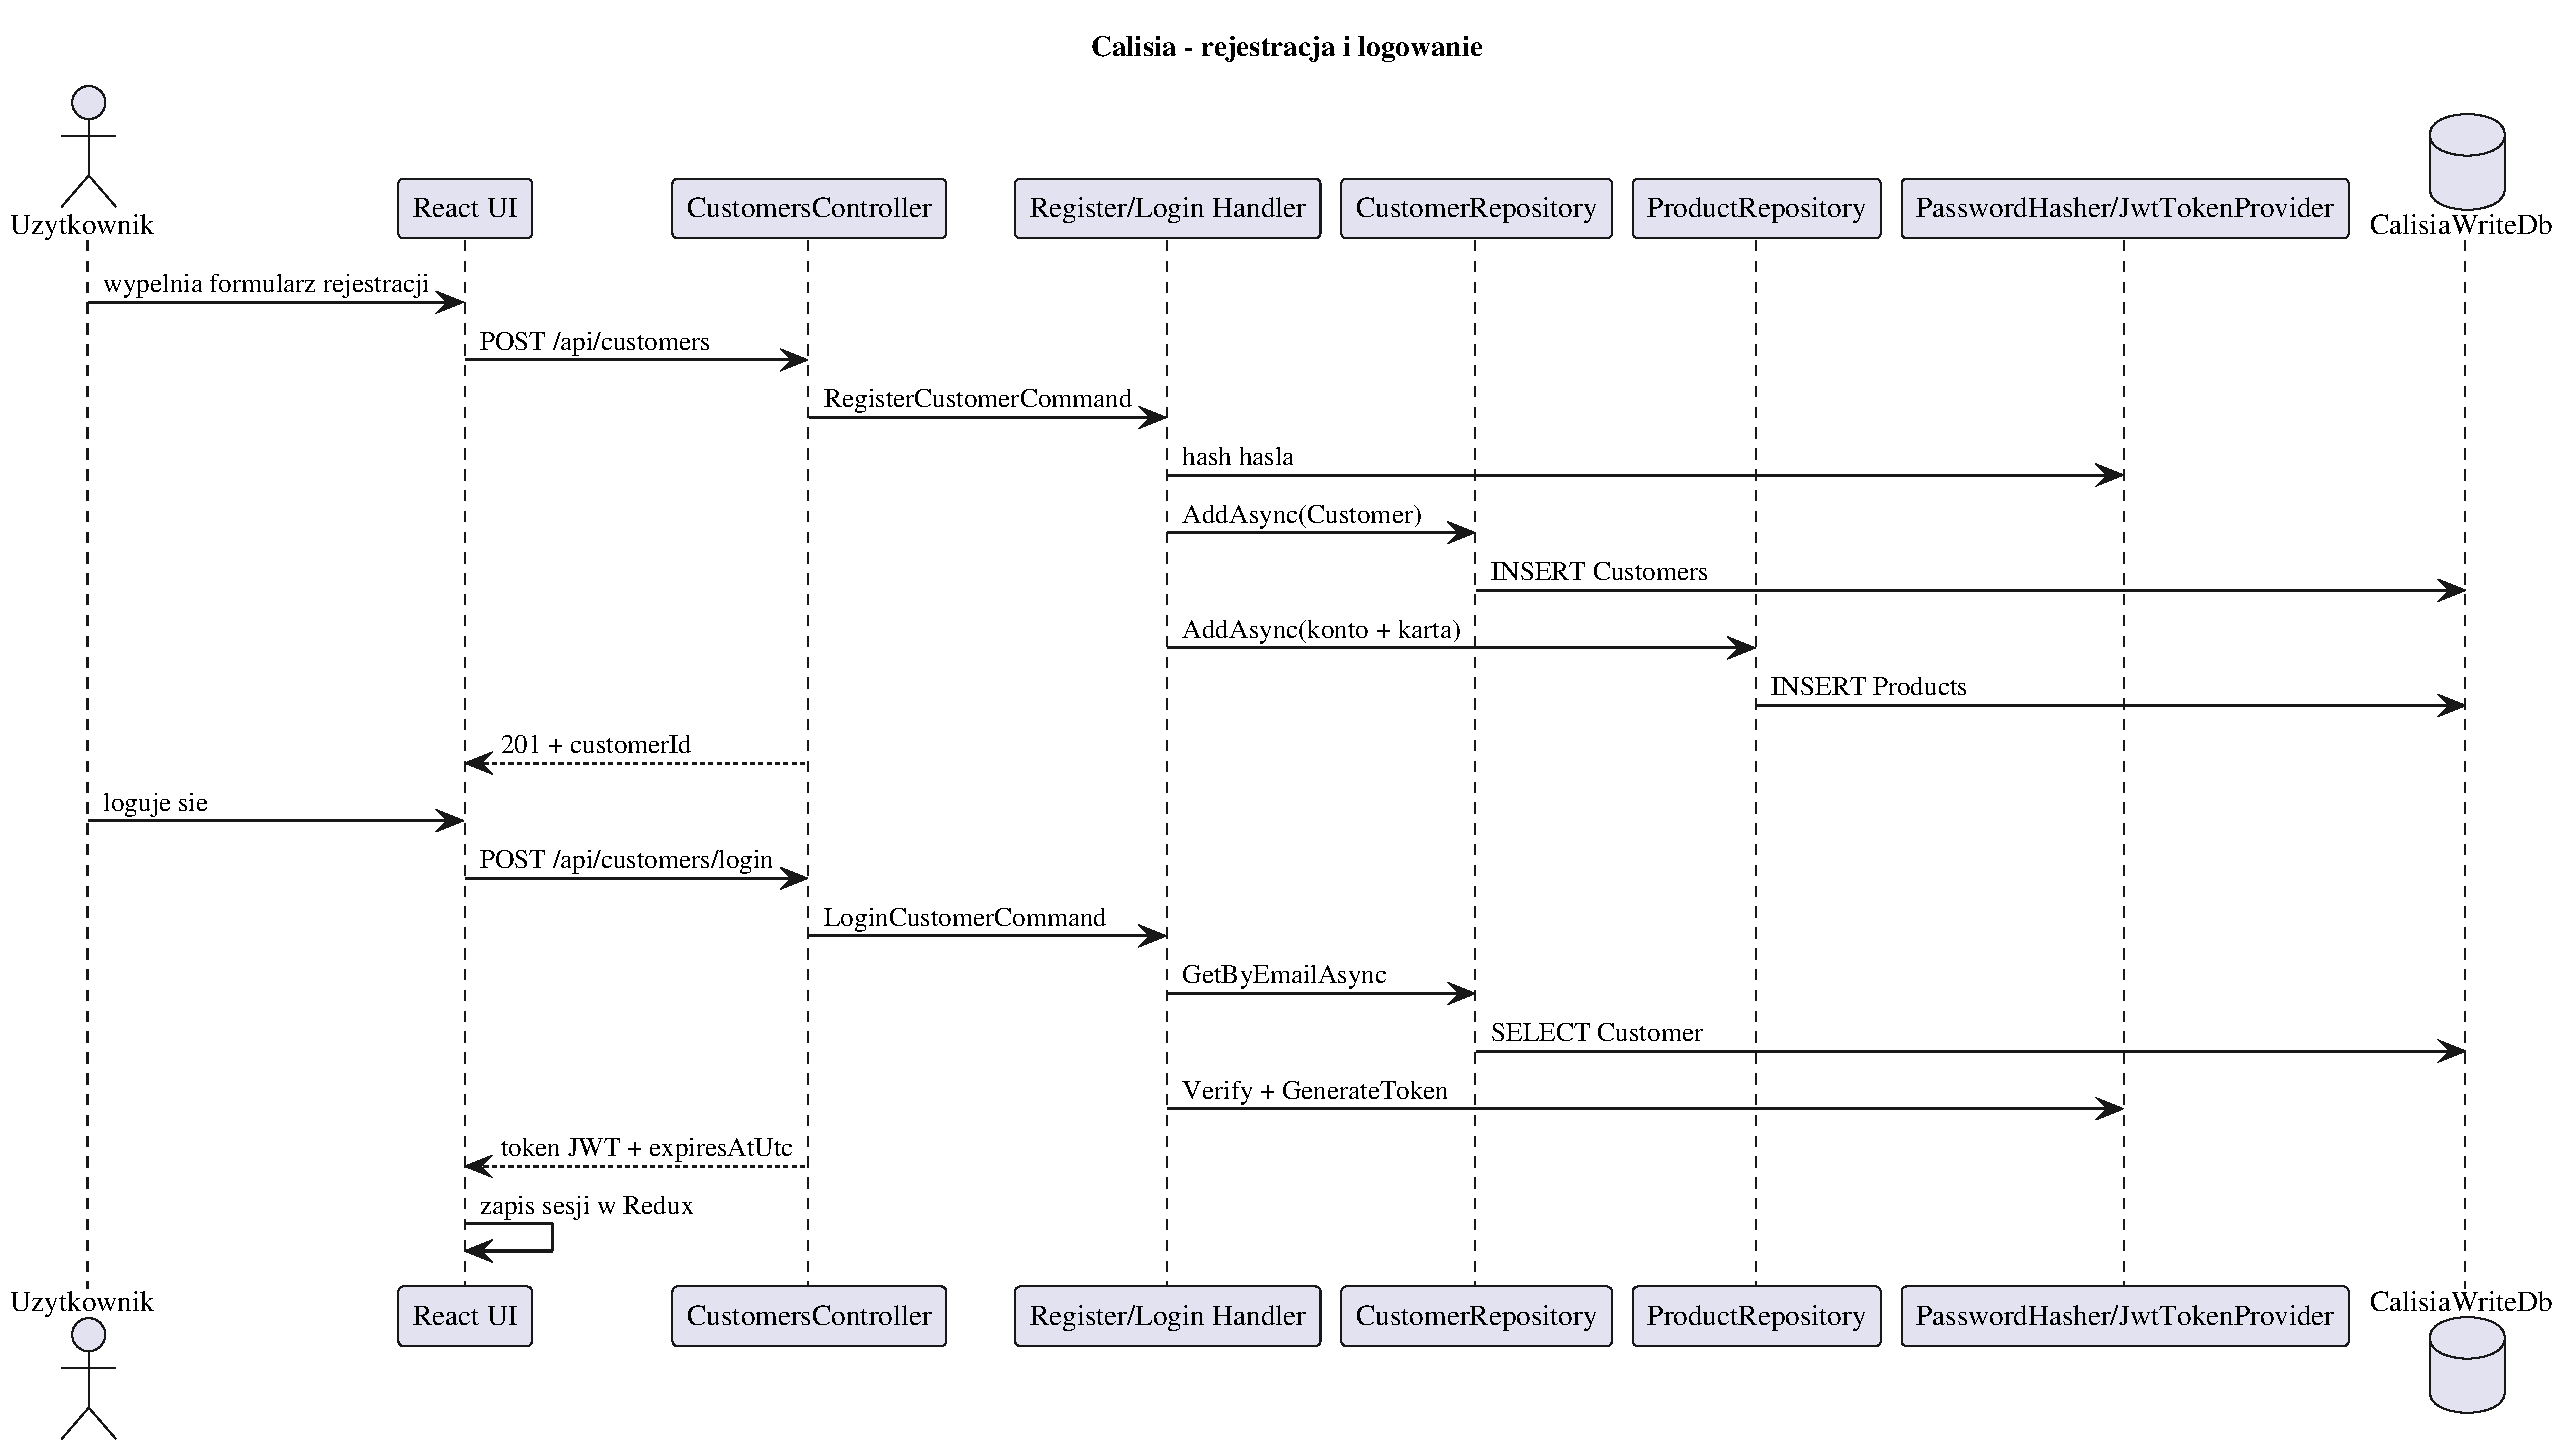
\includegraphics[width=\textwidth,height=0.78\textheight,keepaspectratio]{uml/07_sekwencja_rejestracja_logowanie.pdf}
\caption{Sekwencja rejestracji i logowania}
\opis{Diagram opisuje przejście od formularza rejestracji przez utworzenie klienta i produktów startowych do logowania JWT.}
\end{figure}

\subsection{Przelew i dashboard}

\begin{figure}[H]
\centering
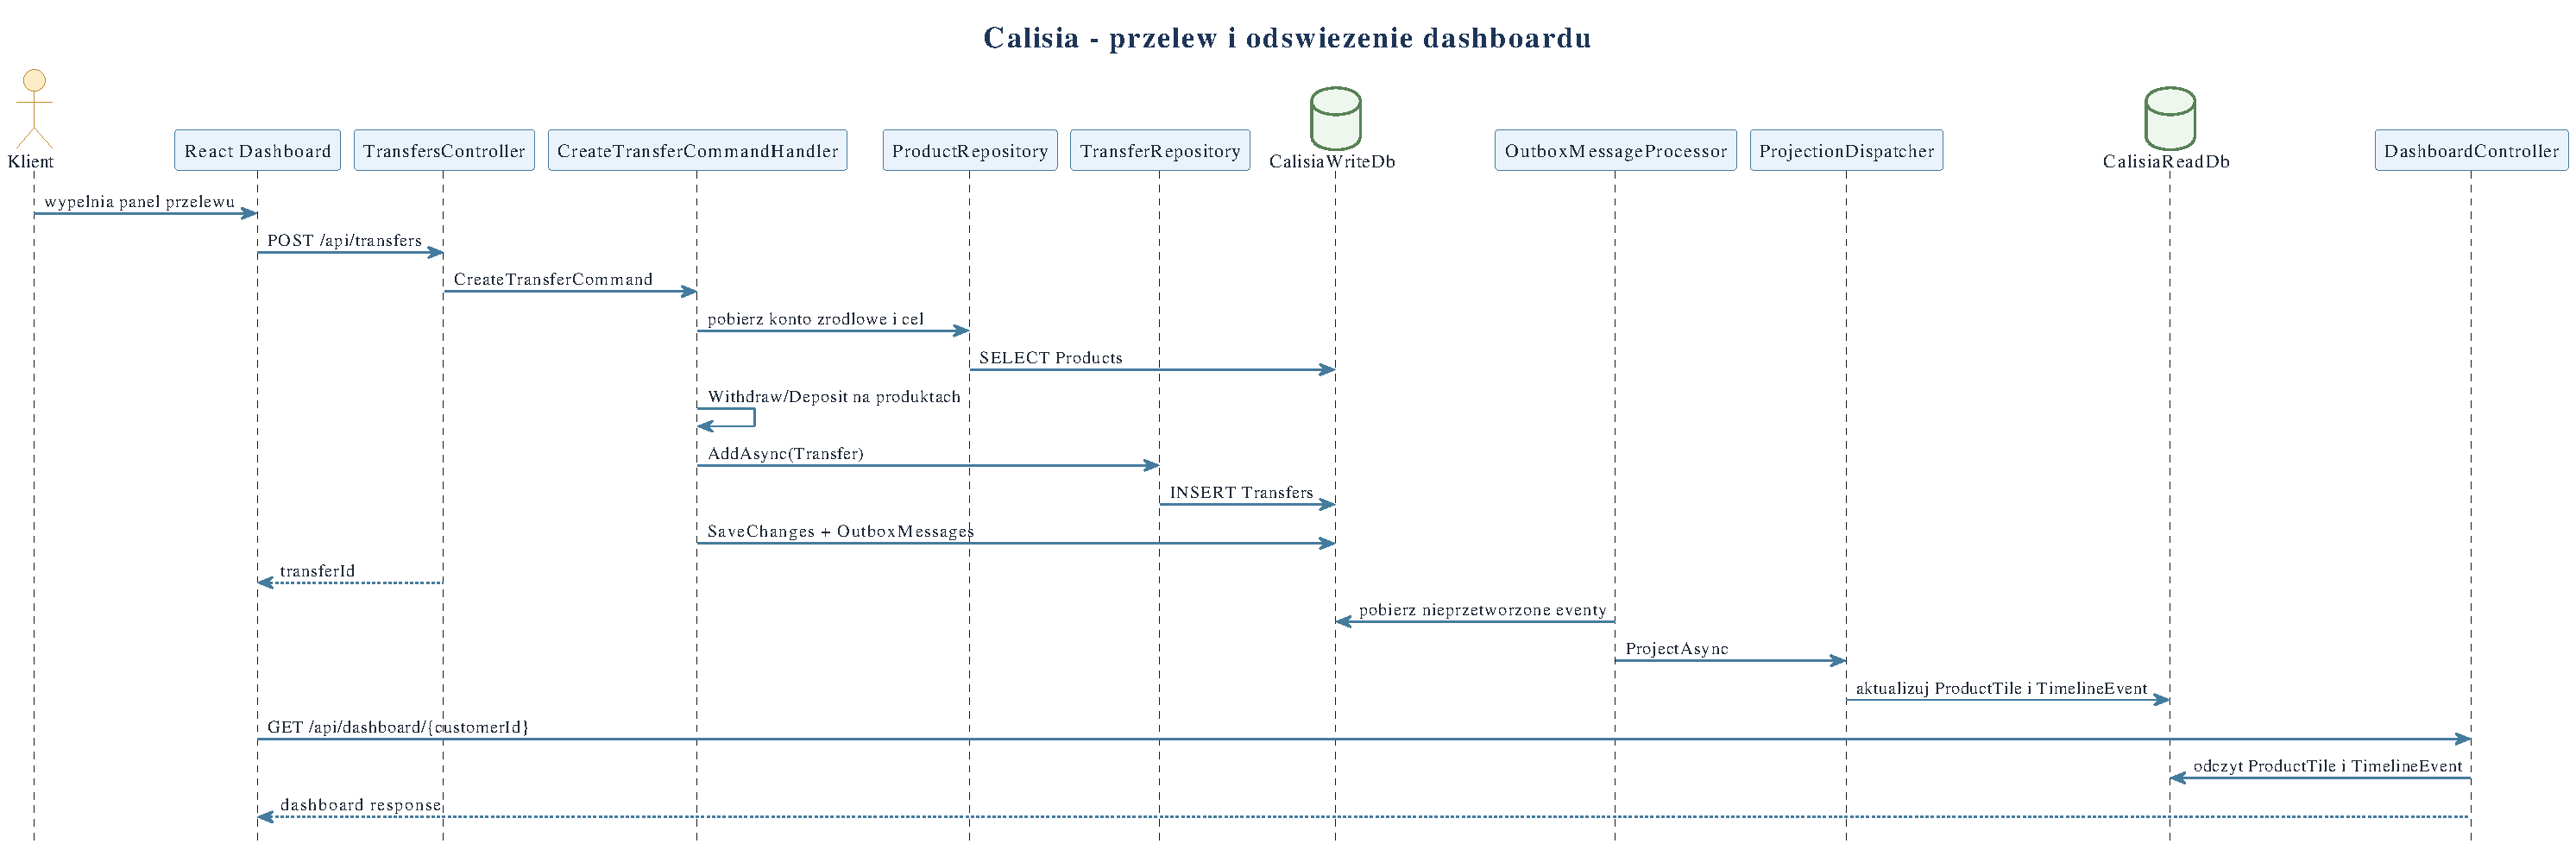
\includegraphics[width=\textwidth,height=0.78\textheight,keepaspectratio]{uml/08_sekwencja_przelew_i_dashboard.pdf}
\caption{Sekwencja przelewu i odświeżenia dashboardu}
\opis{Diagram pokazuje zapis przelewu w modelu write, publikację zdarzeń outbox i odświeżenie modelu read używanego przez dashboard.}
\end{figure}

\subsection{Kredyt i operacje kartowe}

\begin{figure}[H]
\centering
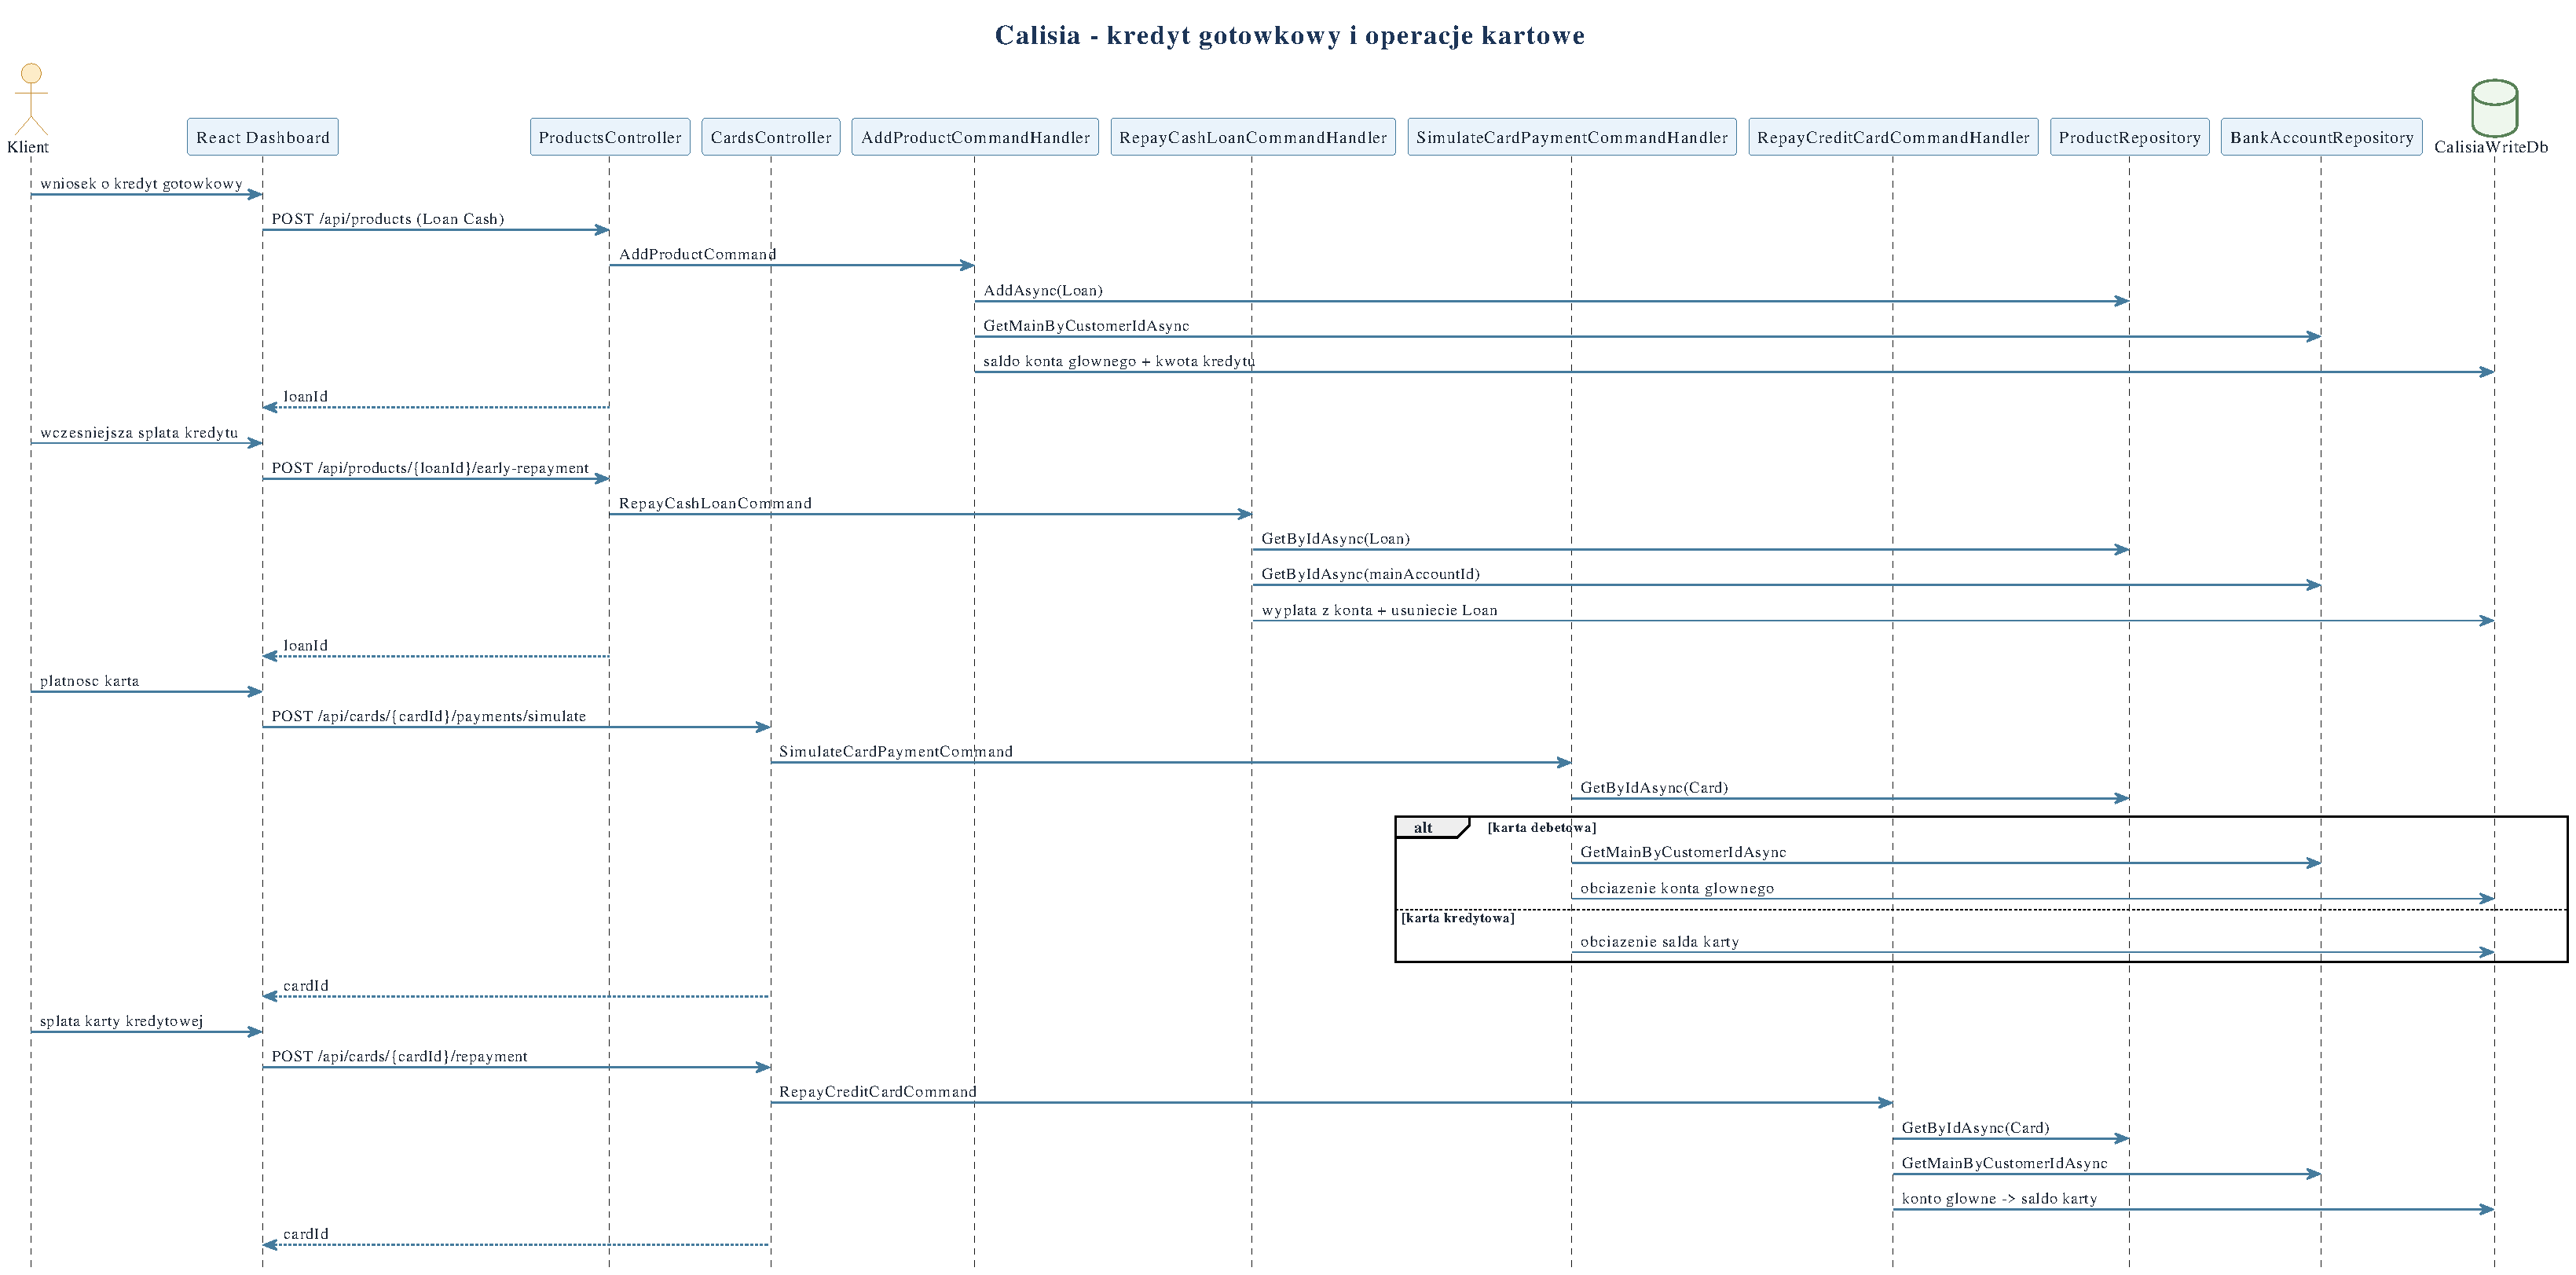
\includegraphics[width=\textwidth,height=0.78\textheight,keepaspectratio]{uml/09_sekwencja_kredyt_i_karty.pdf}
\caption{Sekwencja kredytu gotówkowego i operacji kartowych}
\opis{Diagram zestawia najważniejsze procesy finansowe: uruchomienie i spłatę kredytu, płatności kartą oraz spłatę karty kredytowej.}
\end{figure}

\section{Mechanizm CQRS i Outbox}

W systemie zastosowano rozdzielenie zapisu i odczytu. Komendy modyfikujące stan działają na bazie \texttt{CalisiaWriteDb}. Zdarzenia domenowe są zapisywane jako wiadomości w tabeli \texttt{OutboxMessages}. Procesor outbox przekazuje je do \texttt{ProjectionDispatcher}, który aktualizuje model odczytu.

Takie rozwiązanie pozwala:
\begin{itemize}
\item utrzymać bogaty model domenowy po stronie zapisu,
\item uprościć odczyt danych dashboardu,
\item ograniczyć ryzyko utraty zdarzeń dzięki zapisowi eventów w tej samej transakcji co zmiana domenowa,
\item wykonywać projekcje idempotentnie dzięki tabeli \texttt{ProcessedOutboxMessage}.
\end{itemize}

\section{Bezpieczeństwo}

Autoryzacja użytkownika oparta jest o token JWT. Po zalogowaniu frontend zapisuje token i przekazuje go w nagłówku \texttt{Authorization: Bearer ...}. Endpoint dashboardu dodatkowo sprawdza, czy identyfikator klienta w adresie odpowiada klientowi z tokenu.

Hasła nie są przechowywane jawnie. Backend używa hashera PBKDF2, a w bazie przechowywany jest wynik hashowania. Middleware obsługi wyjątków mapuje błędy domenowe i aplikacyjne na odpowiedzi HTTP.

\section{Testy i narzędzia}

Projekt zawiera testy jednostkowe oraz integracyjne backendu. Testy jednostkowe pokrywają między innymi:
\begin{itemize}
\item tworzenie produktów bankowych,
\item kredyt gotówkowy i jego spłatę,
\item płatności kartą debetową i kredytową,
\item spłatę karty kredytowej,
\item przelewy,
\item hashowanie haseł i tokeny JWT,
\item projekcje modelu odczytu.
\end{itemize}

Do ręcznego testowania endpointów przygotowano kolekcję Bruno. Zawiera ona żądania dla klientów, dashboardu, produktów, przelewów oraz kart.

\section{Wnioski}

Calisia Banking App jest aplikacją demonstracyjną pokazującą bankowość elektroniczną z wyraźnym podziałem warstw, modelem domenowym oraz odseparowanym modelem odczytu. Najważniejszą cechą architektury jest połączenie DDD, CQRS i outbox, które umożliwia spójne przetwarzanie zdarzeń finansowych oraz szybkie prezentowanie danych dashboardu.

Frontend zapewnia użytkownikowi prosty przepływ od rejestracji i logowania po codzienną obsługę rachunku, produktów, kart, kredytu oraz historii operacji. Backend koncentruje reguły biznesowe w domenie i udostępnia je przez czytelne endpointy REST.

\end{document}
